\documentclass[12pt]{article}
\usepackage{evolution}
\usepackage{amsmath}
\usepackage{wrapfig}
%MBE or Evolution

\begin{document}
\linenumbers

%--------------------------------------------------
% Title page
%--------------------------------------------------

\begin{center}
\textbf{The Probability of Sex Autosome Fusions}
\end{center}

\vfill
\noindent
\textit{Running title:} SA-fusions

\vfill
\noindent
Nathan W. Anderson and Heath Blackmon

\noindent
Department of Biology; Texas A\&M University; College Station, TX 77843, USA

\vfill


%--------------------------------------------------
% Abstract, Keywords
%--------------------------------------------------

\noindent
Author for correspondence: HB, \textit{coleoguy@gmail.com}
\vfill

\clearpage


ABSTRACT GOES HERE


\bigskip
\noindent
\textit{Keywords: sexual antagonism; chromosome fusion; sex determination systems; chromosome number}




%--------------------------------------------------
% Introduction
%--------------------------------------------------



\section{Introduction}

The fusion and fission of chromosomes are two of the primary mechanisms that restructure the genome into discrete chromosomes \citep{blackmon2019}.
Early on, it was recognized that both of these changes might be selectively favoured because they modify linkage among loci \citep{white1977,stebbins1971}.
In particular, the fusion of a sex chromosome and an autosome (SA-fusion) has been proposed to resolve sexual antagonism and, therefore, these fusions are predicted to be more common than autosome autosome fusions (AA-fusions) \citep{charlesworth1980}.
Limited empirical examples have shown instances where autosomes which have recently fused with sex chromosomes are enriched for sexual antagonistic loci \citep{zhou2012}.
Furthermore, empirical studies suggest that sexual antagonism may be common throughout the genome \citep{innocenti2010sexually,cheng2016sex}.
However, there remains significant debate as to the ubiquity of sexually antagonistic variation \citep{kasimatis2019limits,ponnikas2018sex}.
A strong measure of the frequency of significant sexually antagonistic variation across the genome would be an excess of SA-fusions relative AA-fusions across large clades.

The probability of SA-fusions is a function of the sex chromosome system and the number of autosomes in the genome.
To facilitate tests of the balance between SA-fusions and AA-fusions, we have derived a closed form equation for the probability of an SA-fusion under a null model where any chromosome is equally likely to fuse with any other non-homologous chromosome.
Our result is applicable to XO, XY and multi-XY (e.g. XXY or XYY) sex determination systems and, with slight modification, to ZW systems.

%--------------------------------------------------
% Model
%--------------------------------------------------

\section{The Model}
% add intro sentence
We ignore fusions among homologous chromosomes, including fusions that join an X and Y chromosome, because this would lead to unbalanced gametes during meiosis and presumably these would be non-viable.
For simplicity, we first examine the case where fusions have equal probability of occurring in males and females, though we show how unequal probabilities can be accommodated.
We begin with the most intuitive case, an XY sex chromosome system, and then proceed to generalize this result to more complex sex chromosome systems.

\subsection{XY System}
When any two chromosomes fuse, there are 3 possibilities. 
The two chromosomes could both be autosomes, they could both be sex chromosomes, or one could be a sex chromosome and the other an autosome. 
We will denote our three possibilities, AA-fusion, SS-fusion, and SA-fusion as events $AA$, $SS$, and $SA$, respectively. 
We are interested in the third possibility, SA-fusion. Unfortunately, this proves difficult to calculate directly. We can avoid this using the complement rule. 
We define the probability of SA-fusion as
\begin{equation} \label{eq1}
P(SA)=1-P(AA)-P(SS)
\end{equation}
We now calculate $P(AA)$ and $P(SS)$ using counting.
%We assume the first chromosome involved in the fusion is 'chosen' independently of the second chromosome involved in the fusion. 
%We can calculate the probability that either chromosome is an autosome or a sex chromosome, then, by independence, we can calculate the probability that both are autosomes as the product of their individual probabilities.
% HB I dont think the two above sentences actually add anything we need to the explanation of the model
We begin with the probability of an AA-fusion, $P(AA)$.
Because we assume every chromosome is equally likely to be 'chosen' to fuse, we can calculate the probability that an autosome is 'chosen' first, $P(A_1)$, as the ratio of the number of autosomes to the total number of chromosomes. 
$P(A_1) = \frac{D_a}{D}$, where $D_a$ is the diploid autosome number and $D$ is the total diploid number.
The probability that the second chromosome involved in the fusion is also an autosome, $P(A_2)$, can be found in a similar manner.
However, the first chromosome cannot be 'chosen' again to fuse with itself, nor can its homolog be 'chosen'. 
So, the number of autosomes available to be 'chosen' is $D_a - 2$, the number of autosomes minus the one already chosen and its homolog.
Similarly, the total number of chromosomes available is $D - 2$. 
Thus, $P(A_2) = \frac{D_a - 2}{D - 2}$, and, by independence, we have $P(AA) = \frac{D_a}{D} \cdot \frac{D_a - 2}{D - 2}$.

Next, we calculate the probability of an SS-fusion. 
Our assumption is that, a chromosome cannot fuse with itself, nor with its homolog. 
In an XY system, there are only two sex chromosomes. 
There is an X chromosome and either a homologous X (in females) or a homologous Y (in males).
Because the sex chromosomes in an XY system are a single pair of homologs, an SS-fusion cannot occur and can be ignored. 
We will revisit this later under multi-XY sex chromosome systems.

Therefore, we find the probability of an SA-fusion in an XY sex chromosome system, $P(SA_{XY})$, is:

\begin{equation} \label{eq2}
    P(SA_{XY}) = 1 - P(AA) - P(SS) = 1 - \frac{D_a}{D} \cdot \frac{D_a - 2}{D - 2}
\end{equation}

\subsection{X0 System}
Equation \ref{eq2} does not extend to an XO system because of differences in the sex chromosome complement of males and females. 
In this system, males have a single X chromosome with no homolog, and females have a pair of homologous X chromosomes. 
The lack of a homolog in males causes males and females to have different diploid numbers and requires us to consider males and females separately. 

We begin with females. Following the same logic as above, we calculate the probability that an autosome is 'chosen' as the ratio of the number of autosomes to the total number of chromosomes present in females. 
$P(A_1) = \frac{D_a}{D_d}$, where $D_d$ is the diploid number in dams. 
The probability that the second chromosome involved in the fusion is also an autosome can be found as the ratio of the number of autosomes available to be 'chosen', $D_a - 2$, the number of autosomes minus the autosome already chosen to fuse and its homolog, and the total number of chromosomes available, $D_d - 2$. 
Therefore, $P(A_2) = \frac{D_a - 2}{D_d - 2}$. 
After employing independence and equation \ref{eq2}, we find a very familiar equation for the probability of a SA-fusion in X0 females $P(SA_d)$ yielding. 
\begin{equation} \label{eq3}
    P(SA_d) =  1 - \frac{D_a}{D_d} \cdot \frac{D_a - 2}{D_d - 2}
\end{equation}
The male case $P(SA_s)$ follows similarly. and we find a nearly identical expression.
The only modification required is to replace $D_d$ with $D_s$, the diploid number of sires, in the denominator.
\begin{equation} \label{eq4}
    P(SA_s) = 1 - \frac{D_a}{D_s} \cdot \frac{D_a - 2}{D_s - 2}
\end{equation}
As in the XY system, we can ignore the possibility of an SS-fusion in both sexes, because every sex chromosome in an individual are homologous in an X0 sex determination system.

Because we assume that males and females make equal contributions to possible fusions, we calculate the probability of a SA-fusion as the average of the probabilities that such a fusion occurs in either sex.
    \begin{equation} \label{eq5}
        P(SA_{X0,XY}) = 1 - \frac{D_a  (D_a - 2)}{2 D_d  (D_d - 2)} - \frac{D_a  (D_a - 2)}{2 D_s  (D_s - 2)}
    \end{equation}
Note that in an XY system (where $D_s = D_d$), the two fractions will combine and equation \ref{eq5} will simplify into equation \ref{eq2}. 
Hence, this result is accurate for both X0 and XY sex chromosome systems.
 
\subsection{XXY System}
Recall in equation \ref{eq1}, we stated that $P(SA) = 1-P(AA)-P(SS)$ in the preceding cases we have been able to ignore the last term, $P(SS)$.
This is not the case in multi-XY systems.
For example, in the XXY system females have four X chromosomes (two homologous pairs) and males have two non-homologous X chromosomes and a Y chromosome.
So, in order to modify equations \ref{eq5} for an XXY system, we must find an expression for the probability of SS-fusion in both males and females. 
In an XXY system females and males have different diploid numbers, so we begin again by considering the male and female cases separately. 

Females in an XXY system will have four X chromosomes, two homologous pairs, and $D_a$ autosomes. 
We calculate the probability of a SS-fusion as the product of the probability of a sex chromosome being 'chosen' to fuse first, $P(S_1)$, and the probability of a sex chromosome being 'chosen' to fuse second, $P(S_2)$. 
Proceeding by counting, we calculate the probability that a sex chromosome is 'chosen' first,
$P(S_1) = \frac{2X_s}{D_d} $, where $X_s$ is the number of X chromosomes present in sires. 
The use of $2X_s$ in females takes advantage of the fact females always have twice as many X chromosomes as males and avoids the use of another variable for the number of X chromosomes in females.
The probability that the second chromosome involved in the fusion is also a sex chromosome can be found in the same manner. 
The number of sex chromosomes available to be 'chosen' is $2X_s - 2 $, the number of X chromosomes minus the one already chosen to fuse and its homolog, and the total number of chromosomes available is $D_d - 2$. 
It follows $P(S_2) = \frac{2X_s-2}{D_d-2}$. 
Therefore, we find the probability of a SS-fusion in females is  $P(SS_d) = \frac{2X_a}{D_d} \cdot \frac{2X_s-2}{D_d-2}$.
Appending this result to the first of equations \ref{eq3}, we find the probability of a SA-fusion in females is:
    \begin{equation} \label{eq6}
        P(SA_d) = 1 - \frac{D_a}{D_d} \cdot \frac{D_a - 2}{D_d - 2} -  \frac{2X_s}{D_d} \cdot \frac{2X_s-2}{D_d-2} = 1 - \frac{D_a(D_a-2) + 2X_s(2X_s-2)}{D_d(D_d-2)}
    \end{equation}

XXY males have two non-homologous X chromosomes a single Y chromosome, and $D_a$ autosomes. 
We assume that the Y chromosome cannot fuse with either of the X's, because of our assumption with regard to fusions of homologous chromosomes. 
The only possible SS-fusion is between the two non-homologous X chromosomes. 
So, we calculate the probability of a sex sex chromosome fusion as the product of the probability to 'choose' the first X chromosome, $P(X_1)$, and the probability of 'choosing' the second X chromosome, $P(X_2)$. 
We calculate $P(X_1)$ as the ratio of X chromosomes to the total number of chromosomes, $P(X_1) = \frac{X_s}{D_s}$.
We calculate $P(X_2)$ as the ratio of the number of remaining X chromosomes ($X_s - 1$ only the single X chosen must be accounted for since it has no homologous X that could be chosen) and the total number of chromosomes available to fuse ($D_s - 2 $, every chromosome except for the X that was picked and the Y).  
Therefore, $P(X_2) = \frac{X_s - 1}{D_s - 2}$ and the probability of a sex sex chromosome fusion in XXY males is $P(SS_s) = \frac{X_s}{D_s} \cdot \frac{X_s - 1}{D_s - 2}$.
Appending this result to equation \ref{eq4}:
    \begin{equation} \label{eq7}
        P(SA_s) = 1 - \frac{D_a}{D_s} \cdot \frac{D_a - 2}{D_s - 2} - \frac{X_s}{D_s} \cdot \frac{X_s - 1}{D_s - 2} = 1 - \frac{D_a(D_a - 2) + X_s(X_s-1)}{D_s(D_s-2)}
    \end{equation}
To formulate our general expression for XXY, XY and XO systems we average the contribution from males and females and simplify:
\begin{equation} \label{eq8}
P(SA_{XXY, XY, XO}) = 1 -\frac{D_a(D_a-2) + 2X_s(2X_s-2)}{2D_d(D_d-2)} - \frac{D_a(D_a - 2) + X_s(X_s-1)}{2D_s(D_s-2)}
\end{equation}


\subsection{XYY System}
In an XYY system, males have a single X chromosome and two non-homologous Y chromosomes, while females have a single pair of homologous X chromosomes.
In females, there is no possibility of a SS-fusion, because the only sex chromosomes that exist are an X and its homolog. 
Recall that in equation \ref{eq8} the probability of both chromosomes in a fusion being sex chromosomes in a female is captured by the expression $2X_s(2X_s-2)$, in an XYY systems $X_s=2$ and this expression will equal 0. 
Therefore equation \ref{eq8} is appropriate for females in an XYY systems as well.
However, in males an SS-fusion between the two Y chromosomes is possible.
As mentioned previously we again ignore the possibility of either of the Y chromosomes fusing with the X.
The probability of a SS-fusion in males is equivalent to the probability of 'choosing' one Y and then the other. 
Proceeding by counting we find: $ P(SS_s) = P(Y_1) \cdot P(Y_2) = \frac{Y}{D_s} \cdot \frac{Y - 1}{D_s - 2}$ where $Y$ is the number of Y chromosomes in males.
Appending this to equation \ref{eq3} we get:
    \begin{equation} \label{eq9}
        P(SA_s) = 1 - \frac{D_a}{D_s} \cdot \frac{D_a - 2}{D_s - 2} - \frac{Y}{D_s} \cdot \frac{Y - 1}{D_s - 2} = 1 - \frac{D_a(D_a - 2) + Y(Y - 1)}{D_s(D_s - 2)}
    \end{equation}
The difference between equations \ref{eq7} and \ref{eq9} is $X_s$ changes to $Y$. 
Therefore, to generate an expression that is applicable to both XXY and XYY systems we take the maximum value among $X_s$ and $Y$:
    \begin{equation} \label{eq10}
        P(SA) = 1 -\frac{D_a(D_a-2) + 2X_s(2X_s-2)}{2D_d(D_d-2)} - \frac{D_a(D_a - 2) + max(X_s,Y)(max(X_s,Y)-1)}{2D_s(D_s-2)}
    \end{equation}

This formulation is applicable to XO, XY, multi-XY sex chromosome systems.
With regard to multi-XY systems, the current formulation would not apply in the rare case where there are multiples of both the X and the Y chromosome.
It is quite possible that the sexes may make unequal contributions to the fusions entering a species, in this case equation \ref{eq10} can be modified by eliminating the averaging among sexes and the addition of a term $\mu_d$, representing the proportion of fusions that occur in females: 
    \begin{equation} \label{eq11}
        P(SA) = 1 -\mu_d\frac{D_a(D_a-2) + 2X_s(2X_s-2)}{D_d(D_d-2)} - (1-\mu_d)\frac{D_a(D_a - 2) + max(X_s,Y)(max(X_s,Y)-1)}{D_s(D_s-2)}
    \end{equation}

\section{Results and Discussion}
%--------------------------------------------------
% Results and Discussion
%--------------------------------------------------

Although illustrated for male heterogametic systems this formulation can be converted for use in ZW sex chromosome systems as well.
Taking equation 10 and exchanging $D_d$ and $D_s$, replacing $X_d$ with $Z_s$, replacing $Y$ with $W$, and replacing $\mu_d$ with $\mu_s$, we generate an equation that will provide probabilities for Z0, ZW, and multi-ZW systems.
There are several cases where the derived equation will fail.
First, in systems with UV sex chromosomes. 
In these systems, it is the gametophyte stage that occurs as separate males (carrying a V chromosome) and females (carrying a U chromosome) \citep{bachtrog2014sex}.
Second, in systems with multiple X and multiple Y chromosomes (e.g. XXXYY) our formulation will fail to provide accurate probabilities.
However, these systems are exceedingly rare across the tree of life.
Among 14,147 surveyed invertebrates just 0.4\% posses these systems, and the vast majority of these (52 species) are all termites in the order Blattodea \citep{blackmon2017}. 
These sex chromosome systems are equally rare in mammals where they are restricted to two species in Monotremata \citep{ashman2014tree}.

\begin{wrapfigure}{r}{0.5\textwidth} %this figure will be at the right
    \centering
    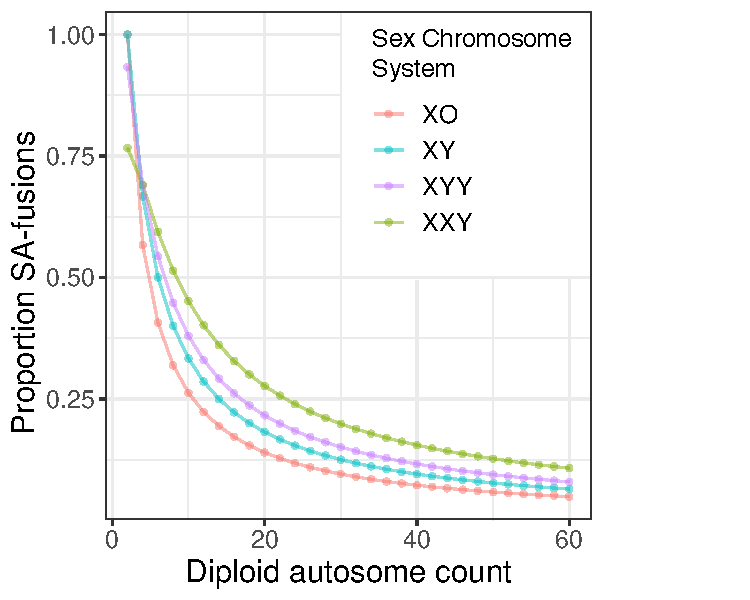
\includegraphics[width=0.45\textwidth]{autosome.num.pdf}
\caption{Probability of a random fusion joining a sex chromosome and autosome. On the vertical axis we plot the proportion of all fusions that are SA-fusions while on the horizontal axis we plot the diploid autosome count. Each sex chromosome system is indicated by a unique color.}
\end{wrapfigure}

The need for a quantitative null model of the proportion of fusions which are SA-fusions is best illustrated by examining the expected proportion across a range of chromosome numbers and sex chromosome systems.
In figure 1, we show when the autosome number is small, a large proportion of fusions is expected to be SA-fusions even under a null model that assumes they are not selectively favored. 
In fact, for the XY sex chromosome system the probability of a random fusion being an SA-fusion does not drop below 25\% until the diploid autosome count is greater than 16. 
In systems with XXY sex determination, the case is even more extreme. The probability of SA-fusion does not go below 25\% until the diploid autosome count reaches 24.

One of the challenges to understanding whether there is an excess of SA-fusions is the relative rarity of these large scale genome rearrangements \citep{blackmon2019}. %and some others
We envision using this equation to calculate the expected proportion of all fusions that are SA-fusions across a clade.
We can do this by leveraging stochastic mappings to extract the proportion of time that lineages in a clade spend with each possible chromosome number and sex chromosome system \citep{huelsenbeck2003, revell2012}.
These proportions can then be used in conjunction with equation \ref{eq10} to generate a weighted sum that describes the expected proportion of all observed fusions that should be SA-fusions (figure 2).
An additional advantage of this approach is that it naturally extends to marginalize over a collection of phylogenetic trees sampled from a posterior distribution.











%--------------------------------------------------
% References
%--------------------------------------------------
\clearpage
\bibliography{refs}
\bibliographystyle{evolution}

\end{document}
